\documentclass[english]{article}
\usepackage[english]{babel} 
\usepackage[T1]{fontenc}
\usepackage[utf8x]{inputenc}
\usepackage{float}
\usepackage{graphicx}

\makeatletter
\usepackage[a4paper,top=2cm,bottom=2cm,left=2cm,right=2cm]{geometry}
\usepackage{enumitem}
\usepackage{subfig}
\usepackage{amsthm}
\usepackage{amsmath}
\usepackage{epstopdf}
\usepackage{fancyhdr}
\usepackage{booktabs,array}

\hyphenation{english}
\makeatother

\usepackage{babel}


\usepackage{listings}
\usepackage{xcolor} % for setting colors

% set the default code style
\lstset{
    frame=tb, % draw a frame at the top and bottom of the code block
    tabsize=4, % tab space width
    showstringspaces=false, % don't mark spaces in strings
    numbers=left, % display line numbers on the left
    commentstyle=\color{gray}, % comment color
    keywordstyle=\color{blue}, % keyword color
    stringstyle=\color{red} % string color
}


\begin{document}
\begin{titlepage}

	\begin{center}
		\begin{Large} \textbf{UNIVERSITY OF PADOVA} \\
		\end{Large} \vspace{1cm}
		\vspace{3cm}
		\begin{Large} Embedded Real--Time Control \end{Large}
		\par\end{center}

	\begin{center}
		\begin{Large}Laboratory report\\
		\end{Large}
		\par\end{center}

	\begin{center}
		\vspace{2cm}
		\begin{figure}[!htb]
			\centering 
\includegraphics[width=8cm]{figures/unipd-logo.png}\\

		\end{figure}

		\par\end{center}

	\begin{center}
		\vspace{2cm}
		\begin{Large} Giulia Cassanego - (2157191), Matteo Mazzocco - (), Davide Pillon - ()  \\
		\end{Large} \vspace{2cm}
		\begin{Large} Academic Year 2024-2025 \end{Large}
		\par\end{center}

\end{titlepage}

\tableofcontents
\newpage

\section{Laboratory 1}
This laboratory focused on practical implementations of serial-bus communication using the I\textsuperscript{2}C protocol, interfacing external devices through the STM32's HAL (Hardware Abstraction Layer). 
The aim was to interface a Pololu QTR reflectance line sensor and a 16-key matrix keypad using two SX1509 I/O expanders connected to the STM32F767 microcontroller through a shared I\textsuperscript{2}C bus. 
The activity covered embedded systems concepts, including interrupt handling, keypad scanning, sensor polling, and dynamic control of an LED.

\subsection{Theoretical background}



% PROBLEM ANALYSIS
% Interfacing multiple I\textsuperscript{2}C slave devices on a shared bus requires managing device addresses, selecting the correct internal registers, and interpreting device-specific data. For real-time responsiveness - such as reacting to a key press - external interrupts are used instead of continuous polling. This lab combined both techniques: polling was used for the line sensor, while interrupts were used for detecting keypad input. 


%Additionally, implementing responsive user interaction through interrupts and traslating raw binary data into usable application logic.

%%%%%%%%%%%%%%%%%%%%%%%%%

\subsubsection{I\textsuperscript{2}C \& HAL Interface}

The Inter-Integrated Circuit (I\textsuperscript{2}C) is a syncronous, multi-master, multi-slave serial communication protocol widely used in embedded systems for short-distance communication. 
It is especially useful when multiple devices share the same bus, as in the case of this laboratory. 
I\textsuperscript{2}C uses two bidirectional lines:

\begin{itemize}
    \item \textbf{SCL} (Serial Clock Line): carries the clock signal generated by the master
    \item \textbf{SDA} (Serial Data Line): transmits and receives data between master and slaves.
\end{itemize}

\noindent
Each I\textsuperscript{2}C communication involves the master initiating a transmission, specifying an address to select a slave device, followed by a read or write operation to specific registers on that device. 
\noindent
To simplify I\textsuperscript{2}C communication, the STM32 HAL (Hardware Abstraction Layer) provides high-level functions that handle the complex low-level protocol mechanics (e.g. generating START/STOP condition, clock stretching and byte-level ACK/NACKs). The two most important functions used in this lab are:


\begin{itemize}
    \item \texttt{HAL\_StatusTypeDef HAL\_I2C\_Mem\_Read()} - to read data from a slave register
    \item \texttt{HAL\_StatusTypeDef HAL\_I2C\_Mem\_Write()} - to write data to a slave register
\end{itemize}

This mechanism was used throughout the lab for example to read the current keypad status and to acquire sensor data from the QTR sensor.


\subsubsection{External Interrupts on STM32}

An interrupt is a hardware-triggered mechanism that suspends the main execution flow, allowing immediate response to input (e.g., key press). In embedded systems, external interrupts are critical for handling asynchronous inputs without polling, improving efficiency and responsiveness. 

STM32 microcontrollers use the EXTI (External Interrupt) peripheral to detect changes on GPIO pins and generate interrupts accordingly. To set up an external interrupts, the target GPIO pin is configured as an input with interrupt capability and the desired trigger edge (rising, falling, or both) is selected. The pin is then mapped to the appropriate EXTI line, the interrupt is unmasked and enabled in the NVIC with a set priority. Once configured, a signal edge on the pin triggers an interrupt that temporarily halts normal execution. STM32'S HAL processes this interrupt through a centralized interrupt service routine (ISR), which subsequently invokes a user-defined callback function: 

\begin{itemize}
    \item \texttt{HAL\_GPIO\_EXTI\_Callback(uint16\_t GPIO\_Pin)}, responsible for handling the interrupt and enabkling the application
\end{itemize}






In this laboratory, an external interrupt was configured on PF4, triggered by SX1509\_2 when a key was pressed on the keypad.


\subsection{System Configuration}
\label{sec:system_configuration}

\begin{itemize}
    \item \textbf{Microcontroller:} STM32F767
    \item \textbf{I\textsuperscript{2}C Bus:}: shared on I2C1
    \begin{itemize}
        \item \textbf{SX1509\_1} (address \texttt{0x3E}): interfaces line sensor interface.
        \item \textbf{SX1509\_2} (address \texttt{0x3F}): serves as the keypad controller.
    \end{itemize}
    \item \textbf{Interrupts:}: the NINT output of SX1509\_2 is connected to PF4 on the microcontroller and configured as GPIO\_EXTI4. This interrupt is triggered on a falling edge when a keypad button is pressed.
    \item \textbf{LED:} connected to PE5, used as output indicator.
\end{itemize}

This laboratory includes structured testing of HAL I\textsuperscript{2}C communication functions and SX1509 registers as detailed in Sections 2.4-2.6 of the handout.

\bigskip


%Two sx1509 are used to interact with the line sensor (Pololu QTR Reflectance Sensor) and with a 16-key keypad. These two devices are connected to the microcontroller through the I2C bus \((\mathbf{I2C\_1})\) and share the same i2c line. Each of them is associated to a different slave address, the first called \( SX1509_1\) is assigned to 0x3E (LINE SENSOR), while the second one \( SX1509_1\) is assigned to address 0x3F (KEYPAD).

%The keypad device is capable of rising an interrupt through the pin NINT which is connected with the pin PF4 (GPIO\_EXTI4\_KPAD\_IR) of the microcontroller STM32F7. 


\begin{figure}[H]
    \centering
    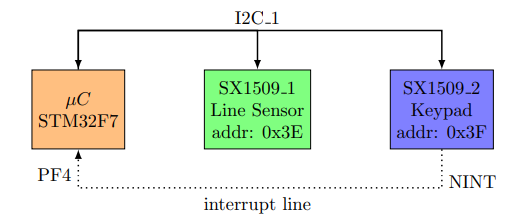
\includegraphics[width=0.55\linewidth]{lab1-2/figures/I2C_scheme.png}
    \caption{I\textsuperscript{2}C connection scheme}
    \label{fig:I2C}
\end{figure}


\subsubsection{Procedure}

In the laboratory setup, to enable the interrupt on pin PF4, the \texttt{*.ioc} configuration file was modified by setting PF4 to \texttt{GPIO\_EXTI4} (GPIO\_EXTI4\_KPAD\_IR). The interrupt trigger mode was configured in \emph{External Interrupt Mode with Falling edge trigger detection}, and the pull-up/pull-down resistors were disabled by selecting \emph{No pull-up and no pull-down}. Additionally, to enable the \texttt{printf} function for debugging purposes, the Serial Wire Viewer (SWV) was activated. 

\subsubsection{SX1509 Register Map}

The SX1509 data registers employed in this lab include: 

\begin{itemize}
    \item \texttt{0x10}: \texttt{REG\_DATA\_B} contains the data of the line sensor
    \item \texttt{0x27}: \texttt{REG\_KEY\_DATA\_1} contains the  status of the column of the keypad (8-bit values)
    \item \texttt{0x28}: \texttt{REG\_KEY\_DATA\_2} contains the  status of the row of the keypad (8-bit values)
\end{itemize}

\subsubsection{Keypad}

A 4x4 matrix keypad is interfaced with the microcontroller through the SX1509\_2 I/O expander, which communicates via the I\textsuperscript{2}C. The Keypad is structured as a matrix composed of 4 rows and 4 columns, resulting in 16 unique keys. Each key press electrically connects a specific row to a specific column, enabling the identification of the key based on its position in the matrix. 

To detect key presses, the SX1509 uses an internal scanning engine. The columns are configured as open drain outputs, while the rows are configured as input with internal pull-up resistors. When a key is pressed, it creates a path to ground between the active column and the corresponding row, causing the associated row input to be pulled low. The idle state (no key pressed), all bits are high (logic '1'), i.e., the register values are 0xFF (255 in decimal). When a  key is pressed, the corresponding bits in both registers are pulled low (logic '0'). Each bit in the register corresponds to a specific row or column, with bit 0 (Least Significant Bit, LSB) representing the first row or column, and subsequent bit representing lines in order. \\

\begin{figure}[H]
    \centering
    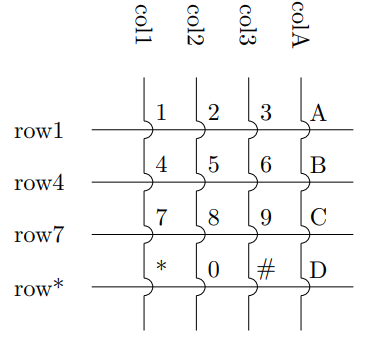
\includegraphics[width=0.45\linewidth]{lab1-2/figures/keypad.png}
    \caption{Keypad scheme}
    \label{fig:keypad}
\end{figure}

\noindent
For example, if the key '8' is pressed (located at row 3, column 2), the SX1509 will return: 

\begin{itemize}
    \item \texttt{REG\_KEY\_DATA\_1} $ =0xFD=0b11111101$ $\rightarrow$ bit 1 (column 2) is low 
    \item \texttt{REG\_KEY\_DATA\_2} $=0XFB=0b11111011$ $\rightarrow$ bit 2 (row 3) is low 
\end{itemize}

\noindent
This binary information allows the software to determine the pressed key by evaluating the position of the zero bits. The microcontroller responds to this event by handling an interrupt (generated on the NINT pin connected to PF4), and reading these two registers using the HAL I\textsuperscript{2}C function \texttt{HAL\_I2C\_Mem\_Read(\&hi2c1, SX1509\_I2C\_ADDR2 << 1, REG\_KEY\_DATA\_1, 1, \&col, 1, I2C\_TIMEOUT)}. The row and column indices are then mapped to a specific character using a predefined lookup table that corresponds to the keypad layout. 

\noindent
This method provides an efficient and reliable way to detect and decode user input from a matrix keypad in embedded systems applications.

%The Keypad is a 4x4 matrix, where each row and column are connected to a set GPIO pins of the device SX1509\_2 using a pull-up resistor. As mentioned above, the status of the key is stored in the registers..
%The least significant bit of the reg1 correspond to the column 1, the second to the column 2 and so on. The same applies to the reg2 ...
%Explain how to understand which key has been pressed...

\subsubsection{Line Sensor (Pololu QTR Reflectance)}
\label{sec:line_sensor}

\noindent
The Pololu QTR reflectance sensor array is a digital infrared sensing system design to detect reflectivity, utilized in Laboratory 4 for line-following applications. It comprises multiple emitter-phototransistor pairs that measure the intensity of reflected infrared light to distinguish between reflective (e.g. white) and non-reflective (e.g. black) surfaces.
In this laboratory setup, the QTR sensor interfaces with the STM32 microcontroller through an SX1509 I/O expander(I2C addres: 0X3E), enabling communication over a shared I\textsuperscript{2}C bus. 
Each sensor in the array operates by charging a capacitor through its phototransistor and then measuring the capacitor's discharge time. On reflective surfaces, the phototransistor saturates, causing rapid discharge and resulting in a short high-pulse duration, interpreted as a logical '1'. Conversely, dark surfaces reflect less infrared light, resulting in slower discharge and longer high pulse, which is thresholded as a logical '0'. This binary abstraction enables digital readout of surface reflectivity:

\begin{itemize}
    \item High (logic 1): White or reflective surface.
    \item Low (logic 0): Black surface.
\end{itemize}


\noindent
The digital outputs of the sensor array are connected to the SX1509's input pins and read the digital state of each sensor line through its register \texttt{REG\_DATA\_B} (address 0x10). The STM32 polls this register using the following HAL function: \\
\texttt{HAL\_I2C\_Mem\_Read(\&hi2c1, SX1509\_I2C\_ADDR1 <<1, REG\_DATA\_B, 1, \&sensor\_line, 1, I2C\_TIMEOUT)}. \\
Each bit in the texttt{sensor\_line} variable corresponds to the the state of an individual sensor element, encoding the presence and relative position of a detected line. This discrete, low-latency data stream provides reliable surface detection, forming the basis for the real-time line-following algorithm implemented in Laboratory 4.


\subsubsection{LED}

The LED used in this experience is connected to pin PE5 (Port E, Pin 5) on the STM32 microcontroller. The LED is directly interfaced with the GPIO through a current limiting resistor (R1), which protects the LED by controlling the current flow. 
The LED is controlled using STM32'S HAL functions. The most relevant function for setting the LED state is: 

\begin{itemize}
    \item \texttt{HAL\_GPIO\_WritePin(GPIOE, GPIO\_PIN\_5, GPIO\_PIN\_SET)}
    \item \texttt{HAL\_GPIO\_ReadPin(GPIOE, GPIO\_PIN\_5)}
    \item \texttt{HAL\_GPIO\_TogglePin(GPIOE, GPIO\_PIN\_5)}
\end{itemize}

This setup allows the LED to be used as a visual indicator in response to GPIO interrupts.


%\subsection{Setup \& Initialization}


\subsection{Code implementation}

--- HAL function - also HAL\_GPIO\_EXTI\_Callback()
    

\subsubsection{Exercise 1 - Keypad interrupt and register read}

An external interrupt callback \texttt{HAL\_GPIO\_EXTI\_Callback()} handles the interrupt from the SX1509 keypad engine on key press (NINT signal). 
The ISR must:

\begin{itemize}
    \item Identify the EXTI pin triggering the event.
    \item Use \texttt{HAL\_I2C\_Mem\_Read()} to read key status registers \texttt{REG\_KEY\_DATA\_1} and \texttt{REG\_KEY\_DATA\_2}.
    \item Print the interrupt source with \texttt{printf()} for debugging feedback.
\end{itemize}

\bigskip

\begin{lstlisting}[language=C]
void HAL_GPIO_EXTI_Callback(uint16_t GPIO_Pin)
{
   // EXERCISE 1

   printf("Interrupt on pin (%d).\n", GPIO_Pin);

   uint8_t col;
   uint8_t row;
   HAL_StatusTypeDef status_col = HAL_I2C_Mem_Read(&hi2c1, SX1509_I2C_ADDR2 << 1, 
   REG_KEY_DATA_1, 1, &col, 1, I2C_TIMEOUT); //col
   HAL_StatusTypeDef status_row = HAL_I2C_Mem_Read(&hi2c1, SX1509_I2C_ADDR2 << 1, 
   REG_KEY_DATA_2, 1, &row, 1, I2C_TIMEOUT); //row

   printf("col = %d\n", col);
   printf("row = %d\n", row);

   ...

}
\end{lstlisting}

\subsubsection{Exercise 2 - Key decoding and display}

In this exercise, we have detect which key was pressed using the cleared bit in column and row readings and then map it using the keypad layout array.

\bigskip

\begin{lstlisting}[language=C]
const char keypadLayout[4][4] = {
    {'*', '0', '#', 'D'},
    {'7', '8', '9', 'C'},
    {'4', '5', '6', 'B'},
    {'1', '2', '3', 'A'}};

void HAL_GPIO_EXTI_Callback(uint16_t GPIO_Pin)
{
   ...
   // EXERCISE 2

   int row_index = -1, col_index = -1;

   // Ogni bit basso (0) rappresenta il tasto premuto
   // 0b11111110 = 254 -bit 0 e' 0, quindi indice 0
   // 0b11111101 = 253 -> bit 1 e' 0, quindi indice 1
   // 0b11111011 = 251 -> bit 2 e' 0, quindi indice 2
   // 0b11110111 = 247 -> bit 3 e' 0, quindi indice 3

   switch (row) {
     case 254: row_index = 0; break;
     case 253: row_index = 1; break;
     case 251: row_index = 2; break;
     case 247: row_index = 3; break;
   }

   switch (col) {
     case 254: col_index = 0; break;
     case 253: col_index = 1; break;
     case 251: col_index = 2; break;
     case 247: col_index = 3; break;
   }

   if (row_index != -1 && col_index != -1) {
     button = keypadLayout[row_index][col_index];
     printf("button = %c \n", button);
   } else {
     printf("Invalid key press: col = %d, row = %d\n", col, row);
   }
   
   ...

}

\end{lstlisting}


\begin{figure}[H]
    \centering
    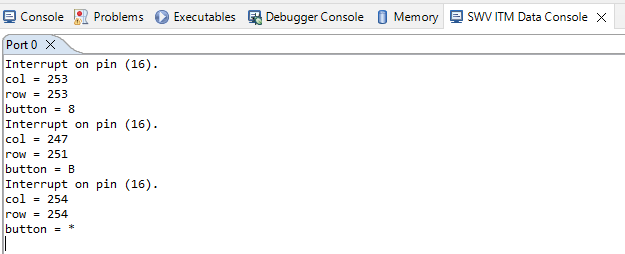
\includegraphics[width=0.75\linewidth]{lab1-2/figures/exercise3.1-3.2.PNG}
    \caption{Printf of the exercise 1-2}
    \label{fig:ex3.2}
\end{figure}


%%%%%%%%%%
%%%%%%%%%%
%%%%%%%%%%
DA RIVEDERE FUNZIONAMENTO KEYPAD
%%%%%%%%%%
%%%%%%%%%%

\subsubsection{Exercise 3 - Line Sensor polling}

In this exercise we need to read the line sensor's state and for doing this we have read the register \texttt{REG\_DATA\_B} using the HAL function \texttt{HAL\_I2C\_Mem\_Read()}. Then we introduce a poll line sensor every 100 ms using \texttt{HAL\_Delay}.

\bigskip

\begin{lstlisting}[language=C]
while (1)
{
    /* USER CODE END WHILE */
    /* USER CODE BEGIN 3 */
    // EXERCISE 3
    
    uint8_t sensor_line;
    HAL_StatusTypeDef status_sens_line = HAL_I2C_Mem_Read(&hi2c1, 
    SX1509_I2C_ADDR1 << 1, REG_DATA_B, 1, &sensor_line, 1, I2C_TIMEOUT);
    printf("status sensor line %d\n", sensor_line);
    HAL_Delay(100);

}

\end{lstlisting}

\subsubsection{Exercise 4 - LED Blinking with dynamic frequency}


(SIMPLE WAY)
\noindent
The key press is captured via the keypad interrupt in \texttt{HAL\_GPIO\_EXTI\_Callback()} and the LED blinking is handled in the while(1) loop.

\bigskip

\noindent
\begin{lstlisting}[language=C]

while (1)
{
    /* USER CODE END WHILE */

    /* USER CODE BEGIN 3 */
   // EXERCIZE 4.1
   if(button < '1' || button > '9'){
     button = '0';
     HAL_GPIO_WritePin(GPIOE, GPIO_PIN_5, GPIO_PIN_RESET);
     continue;
   }
   uint8_t freq = (uint8_t)button - '0';
   HAL_GPIO_TogglePin(GPIOE, GPIO_PIN_5);
   period = 1000/freq;
   HAL_Delay(period/2);

}


\end{lstlisting}


\bigskip
\noindent
(HARD WAY)
We have used the Keypad input to set LED blink frequency. Upon $\#$, the collected digits are converted to an integer. 

%Correct keypress stored in input_buffer[], max three digits. #triggers conversion to integer: target_freq = atoi(input_buffer);
%invalid keys reset the buffer

\bigskip
\noindent
\begin{lstlisting}[language=C]

void HAL_GPIO_EXTI_Callback(uint16_t GPIO_Pin)
{
   ...
   // EXERCISE 4.2

   if (row_index != -1 && col_index != -1) {
     button = keypadLayout[row_index][col_index];
     printf("button = %c \n", button);
     if (button >= '0' && button <= '9') {
       if (input_index < 3) {
         input_buffer[input_index++] = button;
       }
     } else if (button == '#') {
       input_buffer[input_index] = '\0'; // chiusura stringa
       target_freq = atoi((char*)input_buffer); // converte la stringa in intero
       freq_ready = 1;
       input_index = 0; // reset buffer
     } else if (button < '0' || button > '9') {
       // reset se tasto errato o A/B/C/D/*
       input_index = 0;
       target_freq = 0;
       memset((char*)input_buffer, 0, sizeof(input_buffer));
     }
   } else {
     printf("Invalid key press: col = %d, row = %d\n", col, row);
   }

}

\end{lstlisting}

\begin{lstlisting}[language=C]
while (1)
{
   /* USER CODE END WHILE */

    /* USER CODE BEGIN 3 */
   // EXERCISE 4.2

   if (freq_ready && target_freq > 0) {
     uint32_t period = 1000 / target_freq; // periodo in ms
     HAL_GPIO_TogglePin(GPIOE, GPIO_PIN_5);
     HAL_Delay(period / 2); // meta' on, meta' off
   } else {
     HAL_GPIO_WritePin(GPIOE, GPIO_PIN_5, GPIO_PIN_RESET);
     HAL_Delay(100); // idle
   }

}


\end{lstlisting}

\subsection{Results}




\subsection{Conclusion}

This laboratory successfully demonstrated I\textsuperscript{2}C device integration using STM32 HAL, including multi-device communication, external interrupts, register-level control and real-time response to user input. 


\section{Laboratory 2}
%In this laboratory activity, we implemented an open-loop camera system to stabilize a pan-tilt camera mechanism (on a TurtleBot) using IMU data. 

In this laboratory activity, we implemented an open-loop camera stabilization system on a TurtleBot using data from an Inertial Measurement Unit (IMU). The main objective was to maintain a stable field of view for a pan-tilt camera mechanism by compensating for the robot's motion. The stabilization was achieved by calculating tilt and pan angles from the BNO55 IMU sensor and driving two servo motors via the PWM signals. A proportional control strategy was adopted for simplicity and effectiveness, with no position feedback, making it a true open-loop system. Data was logged for further analysis using STM32 and MATLAB. \\
\noindent
This lab introduced key concept such as sensor-based orientation estimation, servo control via PWM, basic proportional controllers and embedded data logging.

%and optional improvement using sensor fusion.

%The exercise involved extracting motion data from the IMU, calculating the tilt and pan angles, and using servo control through PWM signals to realign the camera accordingly. 

\subsection{Problem Analysis}

As TurtleBot moves, its body tilts and pans, causing the camer mounted on the robot to lose its horizontal alignment. This affects the video feed's usability and clarity. The goal is to counteract these motions by adjusting the camera's orientation, ensuring that it remains level with the ground. The key tasks include: 

\begin{itemize}
    \item measuring the robot's motion via accelerometer and gyroscope data.
    \item calculating corresponding tilt (pitch) and pan (yaw) angles.
    \item generating PWM signals to actuate the servo motors and realing the camera.
\end{itemize}

Because the control is open-loop, the system does not read back the actual servo position, so relying on estimated orientation from the IMU.



% USE SENSOR INPUT TO CONTROL SERVO ANGLES FOR CAMERA STABILIZATION
% THE AIMS ARE ESTIMATING ANGLES ACCURATELY USING ACCELEROMETER AND GYROSCOPE DATA, CORRECTLY MAPPING CONTROL SIGNAL TO SERVO PWM VALUES,
%OPERATING WITHOUT FEEDBACK


% When the TurtleBot rotates along the x-axis, the camera tilts with the robot, disrupting a stable wiev. The task is to design a open-loop controller that automatically adjust the tilt servo to counteract the motion and keep the camer level with the horizon. Sensor data from the accelerometer and gyroscope must be processed to derive the current tilt angle and apply corrective control signals to the servo motor.



\subsection{Theoretical background}


%% SPIEGARE METODI PER IL CALCOLO DEL TILT E PAN ANGLE
%% COME MUOVERE LA TELECAMERA CON PWM

\subsubsection{Orientation estimation using IMU}

%BNO55 provides accelerometer and gyroscope data and is used to acquire motion data via I2C. Communication wrappers for reading and writing register are defined using HAL function. 
%bno55_convert_double_accel_xyz_msq()
%bno55_convert_double_gyro_xyz_rps()


From the IMU data, we derive the pitch (tilt) angles, used to orient the camera. There are two main methods used to estimate these angles: 

\begin{itemize}
    \item \textbf{Accelerometer-Based Tilt Estimation}
    
\end{itemize}

\noindent
For the first method we use the y-axis acceleration to compute tilt:

\[\theta = \sin^{-1} \left(\frac{a_y}{g}\right) \]

where $\theta$ is the tilt angle, $a_y$ is the y-acceleration (m/$s^2)$ and $g=9.81 $ $m/s^2$ is the gravitational acceleration.
\noindent
This method is effective for low-frequency, static measurements, but is sensitive to noise and external acceleration.

\bigskip
\begin{itemize}
    \item \textbf{Gyroscope-Based Tilt Estimation}
    
\end{itemize}
\noindent
Instead, if we use this second method, the angular velocity $\omega_x$ from the gyroscope is integrated over time to estimate the tilt angle displacement:

\[\theta_g(t) = \int \omega_x(t) \, dt\]

Then we need to convert it to degrees by multiplying it by 180/$\pi$.

This method accumulates angular displacement over time but suffers from drift due to bias in the gyroscope. 


\subsubsection{Pulse Width Modulation (PWM)}

%Pulse Width Modulation (PWM) is a technique used to simulate analog voltage levels by varying the duty cycle of a digital pulse signal.

Pulse Width Modulation (PWM) is a technique used to simulate analog output using digital signals.
Instead of delivering a constant voltage, PWM controls the amount of power delivered to a device by rapidly switching the signal between high and low states. The key parameter is the duty cycle, which represents the proportion of time the signal stays high within each period.

For example, if the PWM signal has frequency of 50 HZ (i.e. a period of 20 ms), a duty cycle of 50\% means that the signal is high for 10 ms and low for 10 ms within each cycle. By adjusting this ratio, it is possible to control how much effective power is delivered to a device, such as servo motor. 

PWM is widely used embedded systems because it provides an efficient way to control actuators without the need for digital-to-analog converters (DACs). In practice, STM32 hardware timers are configured to generate PWM signals with precise timing and frequency, ensuring stable and responsive control.


%% IMU E SERVO MOTOR

\subsection{System Configuration}

\subsubsection{IMU}


An IMU (Inertial Measurement Unit) is an electronic component used to measure and report an object's linear acceleration, angular velocity and orientation in 3D space. Specifically, we have used: 

\begin{itemize}
    \item a 3-axis accelerometer, which measures linear acceleration along the x, y and z axes.
    \item a 3-axis gyroscope, which measures angular velocity around the same axes.
\end{itemize}

\noindent
These axes are aligned as follows: 

\begin{itemize}
    \item \textbf{x-axis}: pointing to the right
    \item \textbf{y-axis}: pointing backward
    \item \textbf{z-axis}: pointing downwards (towards the ground)
\end{itemize}
%--> TURTLEBOT AXES X, Y, Z

%IMU is equipped with a 3-axis accelerometer that measures linear acceleration and a 3-axis gyroscope that measures the angular velocity in rad/s. 

%HOW IT WORKS ACCELEROMETER AND GYROSCOPE 
\noindent
From the IMU data, we derive the standard Euler angles used in orientation estimation: 

\begin{itemize}
    \item \textbf{Pitch}(Tilt): rotation around the x-axis.
    \item \textbf{Roll}: rotation around the y-axis.
    \item \textbf{Yaw} (Pan): rotation around the z-axis.
\end{itemize}

In our lab setup, tilt refers to the vertical rotation of the camera (pitch), and pan refers to the horizontal rotation (yaw). 

\subsubsection{Servo motor via PWM}

%In this lab, two servo motors were used: one for vertical (tilt) and one for horizontal (pan) adjustment. These servos are controlled through PWM signals generated by the STM32 microcontroller.

In this laboratory, PWM was used specifically to control the position of two servo motors, one for adjusting the til and the other for the pan of a camera mounted on the TurtleBot. Unlike regulare DC motors, which rotate continuously, servos rotate only to a commanded position within a limited range, such as -45° to +45°.

Servo motors interpret PWM signals to determine their target angle. The control signal consists of a PWM signal at a constant frequency, where the pulse width determines the desired angle.

This means the servo expects a PWM signal with a fixed period, where only the duration of the high signal varies. 

To control the servos in our system, we used 
the STM32's Timer 1, which support multiple channels for independent signal generation. 

In this lab setup:

\begin{itemize}
    \item Tilt (Pitch) Servo is connected to TIM1, Channel 3
    \item Pan (Yaw) Servo is connected to TIM1, Channel 2
\end{itemize}

These channels are mapped to specific GPIO pins configured for alternate function mode (AF), enabling them to output the PWM signal generated by TIM1. 

%HAL_TIM_SET_COMPARE()
%saturate()

%The parameters of the PWN and the min and max servo angles were already configured to respect the mechanical constraints without damaging the servos.  
%The PWM is generated using TIM1 and in particular, the tilt is controlled by CHANNER\_3 of TIM1 while the pan is controlled by CHANNEL\_2.

%TO move the camera, we used the following HAL functions:...

%\_\_HAL\_TIM\_SET\_COMPARE is used for setting the compare value for channel 2 and 3 of the TIM1 hardware timer. 



\subsection{Code implementation and Control}

\subsubsection{Tilt Control}

Accelerometer and gyroscope data are read using: 

\begin{lstlisting} [language=C]
bno055_convert_double_accel_xyz_msq(&d_accel_xyz); 
bno055_convert_double_gyro_xyz_rps(&d_gyro_xyz);
\end{lstlisting}

A proportional controller was used to compute the tilt control signal:

\begin{lstlisting} [language=C]

float a_y;
float g = 9.81f;
float K_p_tilt = -1;
float theta_a = 0;

theta_a = asin(a_y/g) * 180.0 / M_PI;// [deg]

tilt = K_p_tilt * theta_a;

\end{lstlisting}


The control signal is then applied to the tilt servo using: 

\begin{lstlisting} [language=C]
_HAL_TIM_SET_COMPARE(&htim1, TIM_CHANNEL_3,(uint32_t)saturate((150+tilt*(50.0/45.0)), 
SERVO_MIN_VALUE, SERVO_MAX_VALUE)); // tilt
\end{lstlisting}

The calculated angle \texttt{tilt} is first scaled to match the corresponding PWM value. This involves mapping the angular range to a range of timer-comparison values that corresponds to the pulse width.  

The mapping used in this laboratory is: 
\begin{lstlisting} [language=C]
(uint32_t)(150+tilt*(50.0/45.0)
\end{lstlisting}

where 150 represents the neutral position, tilt the control input in degrees and 50/45 is a scaling factor to convert $\pm 45$° to $\pm 50$ PWM units. 

To ensure safety, this value is passed through a saturate() function that clamps it within the physical limits of the servo, preventing over-rotation or mechanical damage. 

%The tilt and pan control signals are derived as follows: \\

-- INSERT CODE





\subsubsection{Data logging}

Data logging uses either:

\begin{itemize}
    \item Serial interface via USB (use in this lab)
    \item Wifi datalogger 
\end{itemize}


The matlab commands used to visualize the logged data are:

\begin{lstlisting} [language=matlab]
data = serial_datalog ('COMx', {'3*single','1*single'}, 'baudrate', 115200);
\end{lstlisting}

where 3*single represent accelerometer readings and 1*single the control signal.


The C data structure for logging

\begin{lstlisting} [language=C]

struct datalog
{
    //float accel_x, accel_y, accel_z;
    //float gyro_x, gyro_y, gyro_z;
    float th, control_signal_tilt;
    float ph_g, control_signal_pan;
} logger_data;

\end{lstlisting}

Logging in the main loop:

\begin{lstlisting} [language=C]


    logger_data.accel_x = d_accel_xyz.x;
    logger_data.accel_y = d_accel_xyz.y;
    logger_data.accel_z = d_accel_xyz.z;
    logger_data.gyro_x = d_gyro_xyz.x;
    logger_data.gyro_y = d_gyro_xyz.y;
    logger_data.gyro_z = d_gyro_xyz.z;*/
    
    logger_data.control_signal_tilt = tilt;
    logger_data.control_signal_pan = pan;
    logger_data.th = theta_a;
    logger_data.ph_g = phi_g;
    
    ertc_dlog_update(&logger);//check if some one is connected and waiting for data
    ertc_dlog_send(&logger, &logger_data, sizeof(logger_data));//send data A MATLAB

\end{lstlisting}


\subsection{Results}

Exercise 1 - develop a control law to stabilize the camera's tilt by utilizing data from an IMU.

\subsubsection{Exercise 1 : Tilt Stabilization}

Using the accelerometer-based tilt estimate and a proportional controller, the camera sussfully maintained a level tilt when the TurtleBot was manually tilted forward and backward. The servo responded proportionally to the calculated angle, demonstrating a functioning open-loop stabilization.


\begin{figure}[H]
    \centering
    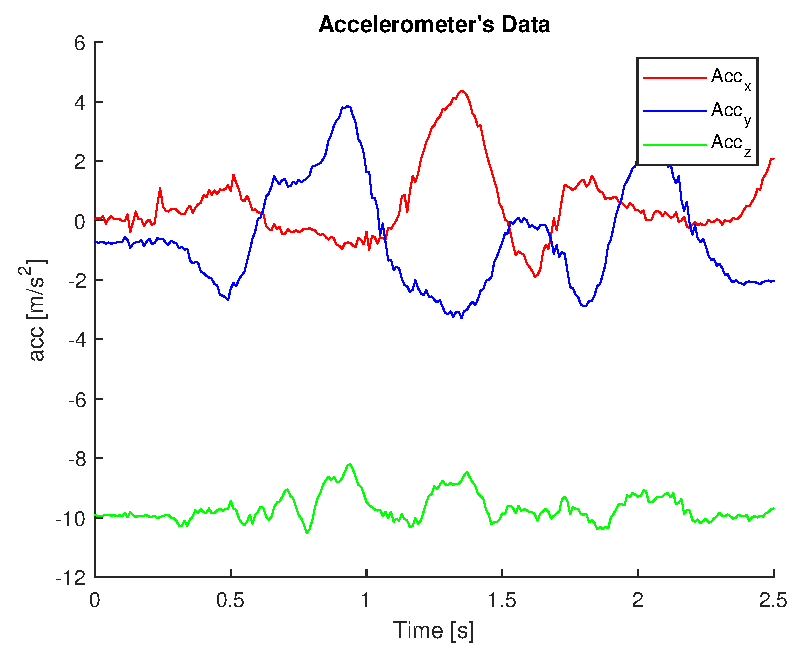
\includegraphics[width=0.5\linewidth]{lab1-2/figures/Accelerometer_Data.eps}
    \caption{Accelerometer data}
    \label{fig:acc_data}
\end{figure}

\begin{figure}[H]
    \centering
    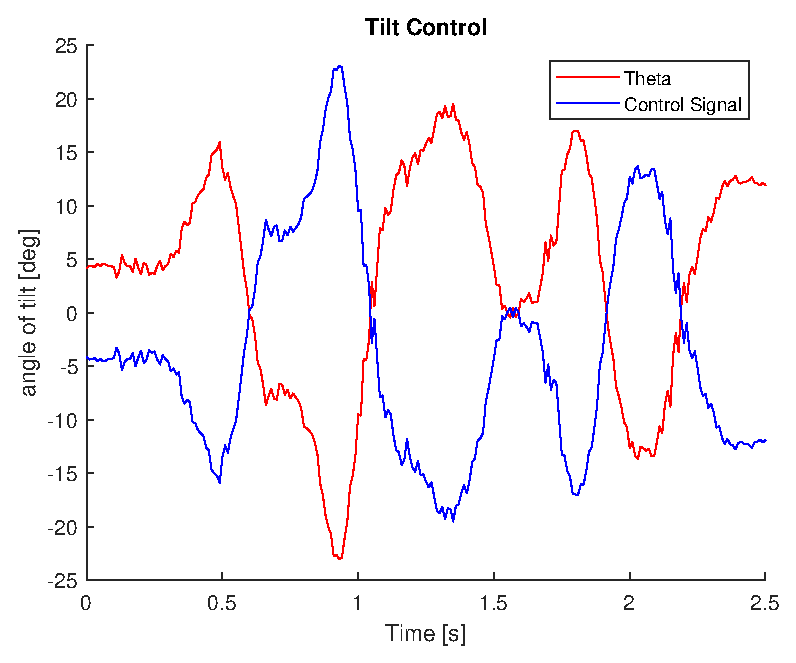
\includegraphics[width=0.5\linewidth]{lab1-2/figures/Tilt.eps}
    \caption{Tilt}
    \label{fig:tilt}
\end{figure}



--- ADD PLOT AND VIDEOS

\subsubsection{Bonus: Smooth Pan Control}

Bonus 1 - control algorithm that implements a "smooth pan" control using data from the gyro.  \\

The pan control using gyroscope data produced a smooth response. Since yaw changes accumulate over time, the camera followed the turning motion of the TurtleBot with a lag defined by the proportional gain.










\section{Laboratory 3}
\input{lab3.tex}

\section{Laboratory 4}
The goal of this laboratory activity was to implement a simple algorithm for line following using our TurtleBot. The robot was equipped with a line sensor array, which allowed it to detect the presence of a line on the ground.
The line sensor array consisted of multiple infrared sensors that could detect the contrast between the line and the background surface. In our case the sensor was placed on the front side of the rover. 
The robot was programmed to follow the line by adjusting its speed and direction based on the sensor readings. 
In particular we implemented two algorithms: 
\begin{itemize}
    \item A simple initial algorithm that used the sensor readings to determine whether the robot was on the line, off to the left, or off to the right. Based on this information, the robot adjusted its speed and direction to stay on the line.
    \item A more advanced algorithm, i.e. the yaw controller, which used the sensor readings to calculate the error in the robot's position relative to the line. The robot then adjusted its speed and direction based on this error, allowing it to follow the line more accurately.
\end{itemize}

\subsection{Model of the robot}
In this section we will describe the model of the robot used in this laboratory activity. In particular, we will focus on the line sensor array and on the kinematic model of the robot.

\subsubsection{Line sensor array}
Our line sensor array consisted of the Pololu QTR reflectance sensors, whose modo operandis is described in Section~\ref{sec:line_sensor}. 
We remind that the microcontroller can read from the reflectance sensor by interfacing with a port expander, which is connected to the sensors via an I2C bus connection.
An important parameter of the sensor line is the pitch, which is the distance between two adjacent sensors. The list below summarizes the main parameters of the sensor array used in this laboratory activity:
\begin{table}[H]
    \centering
    \begin{tabular}{cc}
        \toprule
        \textbf{Parameter} & \textbf{Value} \\
        \midrule
        Sensor output & digital \\
        Number of sensors ($N$) & 8 \\
        Pitch ($P$) & 8 mm or 0.008 m \\
        \bottomrule
    \end{tabular}
    \caption{}
\end{table}

Furthermore, we worked under the following assumptions:
\begin{itemize}
    \item The line is wide enough to activate at least two sensors at a time;
    \item There is always at least one sensor that is not active;
    \item A line is detected if one or more adjacent sensors are activate.
\end{itemize}

For our goal, it was important to define the line tracking error $e_{SL}$, which is the distance between the center of the robot and the center of the line, i.e.
\begin{equation}
    f(x) = \left\{
    \begin{array}{ll}
        e_{SL} = 0 & \text{when the line is at the center} \\
        e_{SL} > 0 & \text{when the line is on the left side of the sensor} \\
        e_{SL} < 0 & \text{when the line is on the right side of the sensor}
    \end{array}
    \right.
\end{equation}
We define the sequence of active sensors as:
\begin{equation}
    b_n = 
    \begin{cases}
        1 & \text{if sensor $n$ is active} \\
        0 & \text{if sensor $n$ is not active}
    \end{cases}
\end{equation}
and the distance between the sensor at position $n$ and the center of the sensor array as:
\begin{equation}
    \label{eq:lambda_n}
    \lambda_n = \left( \frac{N-1}{2} - n \right) \, P, \quad n = 0, \ldots, N-1
\end{equation}
The line tracking error can then be computed as the weighted average of the distances of the activate sensors from the center of the sensor array, i.e.:
\begin{equation}
    \label{eq:e_sl}
    e_{SL} = \frac{\sum_{n=0}^{N-1} b_n \lambda_n}{\sum_{n=0}^{N-1} b_n} 
\end{equation}

\begin{figure} [H]
    \centering
    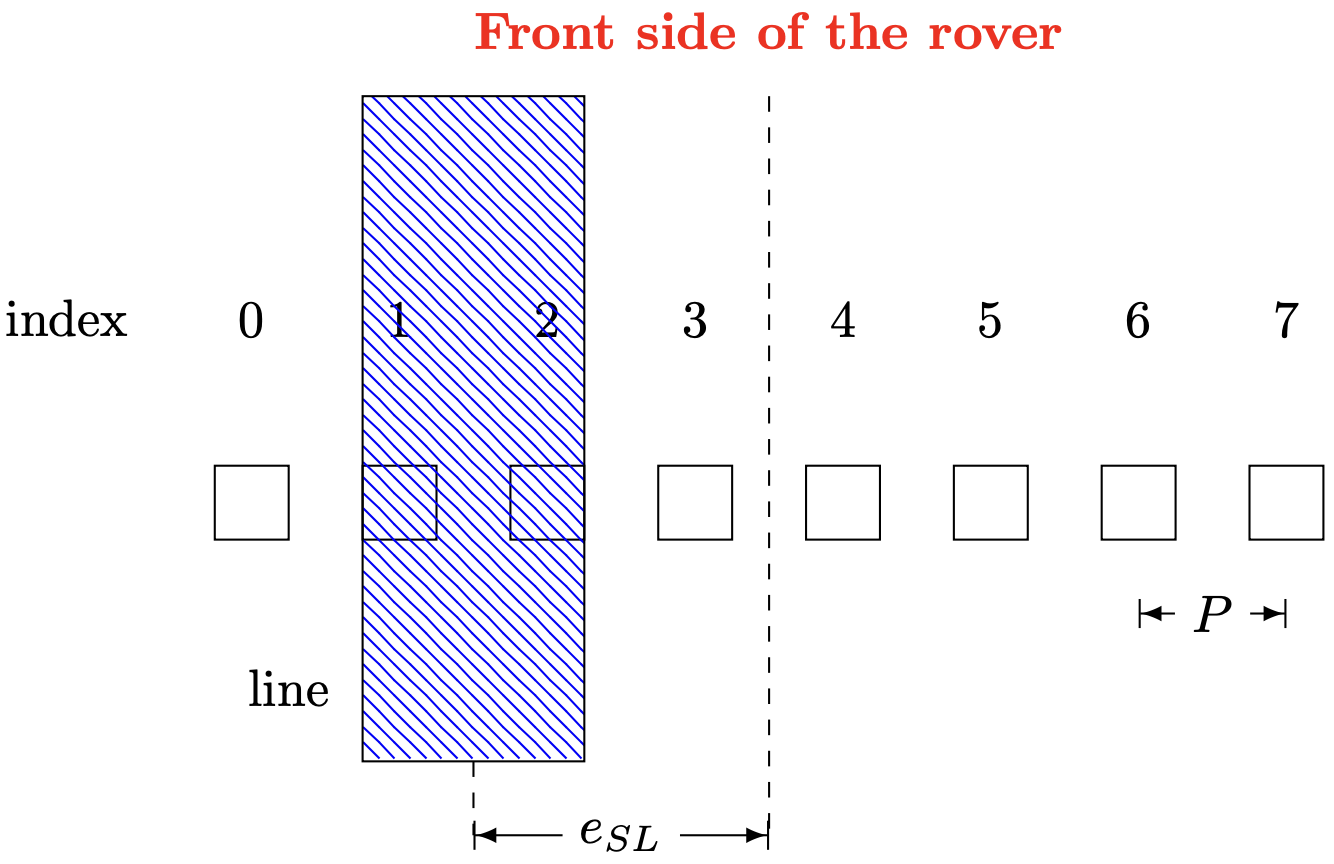
\includegraphics[width=0.7\textwidth]{lab4/figures/e_sl.png}
    \caption{Line tracking error}
    \label{fig:line_tracking_error}
\end{figure}

\subsubsection{Kinematic model}
In Figure~\ref{fig:kinematic_model} is shown the kinematic model of the robot used in this laboratory activity, whose mechanical parameters are reported in Table~\ref{tab: mech_param}.
\begin{table}[H]
    \centering
    \begin{tabular}{cc}
        \toprule
        \textbf{Parameter}  & \textbf{Value} \\
        \midrule
        Wheel distance ($D$) & 0.165 m \\
        Distance between the sensor and the vehicle's centre ($H$) & 0.085 m \\
        Wheel radius ($r$) & 0.034 m \\
        \bottomrule 
    \end{tabular}
    \caption{}
    \label{tab: mech_param}
\end{table}
The robot has two wheels that can be controlled independently, and in the following we assume a pure roll condition, i.e. the wheels do not slip on the ground.
The relations that connect the linear velocity of the wheels $V_l$ and $V_r$ with the angular velocities of the left and right wheels $\omega_l$ and $\omega_r$ are:
\begin{equation}
    V_r = r \cdot \omega_r, \quad V_l = r \cdot \omega_l
\end{equation}
where $r$ is the radius of the wheels.
The rotation of the robot is around the Instantaneous Center of Rotation (ICR), which is the point where the robot is not moving. The ICR is located at a distance $R$ from the center of the robot.
While, the distance between the two wheels is denoted as $D$. It holds that:
\begin{equation}
    V_r = \omega(R+D/2), \quad V_l = \omega(R-D/2)
\end{equation}
and by subtracking these two equations we obtain:
\begin{equation}
    \omega = \frac{V_r - V_l}{D}
\end{equation}

The angle $\psi$ between the global frame and the robot's frame is equal to the angle between the x-axis and the line connecting the ICR to the center of the robot, i.e. $\omega$.
Therefore, the yaw rate of the robot is equal to $\omega$, i.e.:
\begin{equation}
    \dot{\psi} = \frac{V_r - V_l}{D}
\end{equation}
Then, the linear velocity of the robot can be computed as the average of the linear velocities of the two wheels, i.e.:
\begin{equation}
    V = \frac{V_r + V_l}{2}
\end{equation}
And, finally, we derive the formulas which take into account both the longitudinal speed of the wheels and the yaw rate:
\begin{equation}
\begin{cases}
    V_r = V + \dot{\psi} \frac{D}{2} \\
    V_l = V - \dot{\psi} \frac{D}{2}
\end{cases}
\end{equation}
from which it immediately follows
\begin{equation}
\begin{cases}
    \label{eq:omega}
    \omega_r = \frac{V + \dot{\psi} \frac{D}{2}}{r} \\
    \omega_l = \frac{V - \dot{\psi} \frac{D}{2}}{r}
\end{cases}
\end{equation}
\begin{figure} [H]
    \centering
    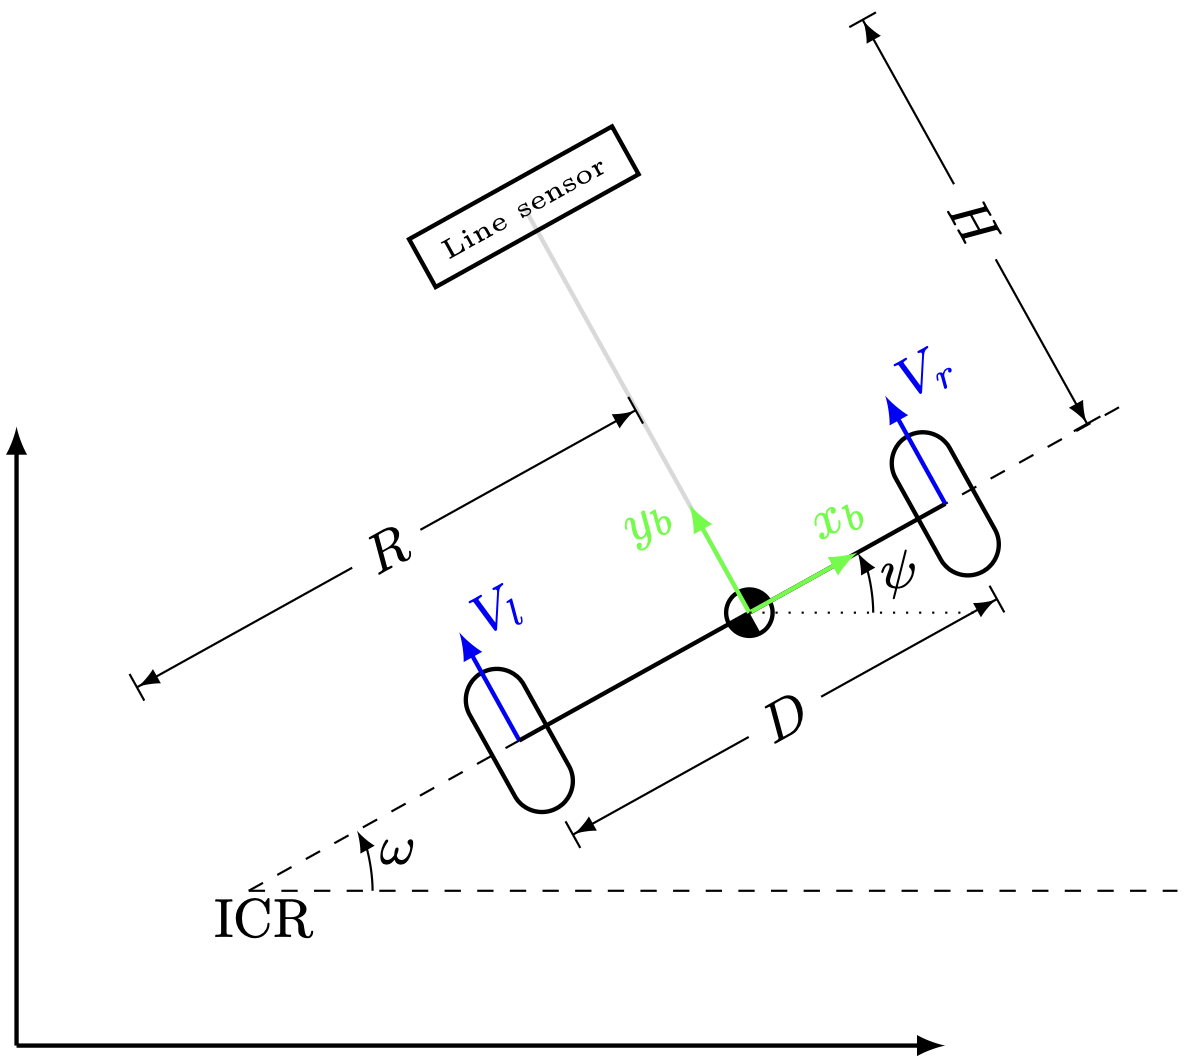
\includegraphics[width=0.6\textwidth]{lab4/figures/kinematic_model.png}
    \caption{Kinematic model}
    \label{fig:kinematic_model}
\end{figure}

\subsubsection{Yaw error}
At this point, we need to define the yaw error, which is the difference between the desired yaw angle ($\psi_{ref}$) and the actual yaw angle ($\psi$) of the robot. The yaw error can be expressed as:
\begin{equation}
    \psi_{err} = \psi_{ref} - \psi
\end{equation}

The relationship between the yaw error and the line tracking error can be expressed as follows:
\begin{equation}
    \label{eq:psi_err}
    \psi_{err} = \arctan\left(\frac{e_{SL}}{H}\right) \approx \frac{e_{SL}}{H}
\end{equation}
Where the last equation exploits the small angle approximation, which is valid for small values of $e_{SL}$.

\subsection{Implementation of the simple controller}
As initial approach we implemented a simple controller with the goal of keeping the robot on the line.
The controller was designed to to adjust the direction of the robot, by increasing the rotation speed of one wheel and decreasing the other, based on the readings of the line sensor array.

The global variables used in the code are shown in Code~\ref{lst:global}. 
These include the speeds of the motors (in RPM), reference values, control errors, and proportional-integral control terms for each motor. 
Gains Kp and Ki are used in the PI controller to regulate the motor speed based on the error. 
Variables are defined separately for motor 1 (controlled via timer 3) and motor 2 (controlled via timer 4).
\begin{lstlisting}[language=C, caption={Global variables}, label={lst:global}]
// motor 1
float TIM3_speed; // Speed of motor 1 in RPM
float reference_speed = 60; //RPM
float speed_error; 
static float u_int; // Integral term for speed control
float u_p; // Proportional term for speed control
float u_pi; // Proportional-Integral term for speed control
float Kp = 0.5;  // Proportional gain
float Ki = 6;    // Integral gain
uint32_t TIM3_CurrentCount;
int32_t TIM3_DiffCount;
static uint32_t TIM3_PreviousCount = 0;
float duty;

// motor 2
float TIM4_speed; // Speed of motor 2 in RPM
float reference_speed2 = 60; //RPM
float speed_error2;
static float u_int2; // Integral term for speed control
float u_p2; // Proportional term for speed control
float u_pi2; // Proportional-Integral term for speed control
float Kp2 = 0.5;  // Proportional gain
float Ki2 = 6;    // Integral gain
uint32_t TIM4_CurrentCount;
int32_t TIM4_DiffCount;
static uint32_t TIM4_PreviousCount = 0;
float duty2;
\end{lstlisting}

First of all, we checked the status of the line sensor, and we saved it in an array, where each element represents the status of a sensor (active [1] or not active [0]).
\begin{lstlisting}[language=C, caption={Status sensor line}, label={lst:sens_line}]
uint8_t sensor_line;
HAL_StatusTypeDef status_sens_line = HAL_I2C_Mem_Read(&hi2c1,
    SX1509_I2C_ADDR1 << 1, REG_DATA_B, 1, &sensor_line, 1, I2C_TIMEOUT);
for (int i = 0; i < 8; i++) {
    if ((sensor_line >> i) & 0x01) {
        active_pins[i] = 1;
    } else {
        active_pins[i] = 0;
    }
}
\end{lstlisting}
% TODO: check se codice c'è già nella parte del lab1

Next, inside the \texttt{HAL\_TIM\_PeriodElapsedCallback(TIM\_HandleTypeDef *htim)} function, we read the array \texttt{active\_pins} and we implemented the simple controller.
We decided to monitor only the pins on the far left (\texttt{active\_pins[0..2]}) and the far right (\texttt{active\_pins[5..7]}) to determine if the robot is drifting off the line.
Based on which pins are active, we adjust the reference speed of one motor to induce a turning behavior (see Code~\ref{lst:simple_alg}).
It is important to note that the \texttt{if} statements are not mutually exclusive, so if multiple conditions are satisfied, the last one overrides the previous ones.
This allows for a graded control based on how far the robot is from the center.
The logic focuses on turning by modifying only one of the two motors. For instance, if the robot needs to turn left, only the speed of motor 2 is increased, while motor 1 remains unchanged (default speed of 0 unless otherwise specified).
\begin{lstlisting}[language=C, caption={Simple algorithm}, label={lst:simple_alg}]
    //turn left
	if(active_pins[0])
		reference_speed2 = 10;
	else if(active_pins[0] && active_pins[1])
		reference_speed2 = 25;
	else if(active_pins[0] && active_pins[1] && active_pins[2])
		reference_speed2 = 37;

	//turn right
	if(active_pins[7])
		reference_speed = 10;
	else if(active_pins[7] && active_pins[6])
		reference_speed = 25;
	else if(active_pins[7] && active_pins[6] && active_pins[5])
		reference_speed = 37;
\end{lstlisting}

To compute the actual motor speed in RPM, we used the \texttt{\_\_HAL\_TIM\_GET\_COUNTER(\&htim3)} function to read the timer value. 
The RPM is calculated using the difference between the current and previous counter values, normalized with respect to the sampling time and the timer resolution.
We calculated the error between the reference speed and the current speed: \texttt{speed\_error = reference\_speed - TIM3\_speed;} for motor 1 and \texttt{speed\_error2 = reference\_speed2 - TIM4\_speed;} for motor 2. 
 This error is used in a PI (Proportional-Integral) controller to generate a control output, as shown in Code~\ref{lst:speed_control}.
The integral term accumulates the error over time, while the proportional term reacts to the current error. The final control output \texttt{u\_pi} is used to adjust the PWM duty cycle sent to the motor.
Note that the integral term \texttt{u\_int} is not bounded or clamped, which may lead to integrator windup if the error persists for a long time. This can be mitigated by adding saturation or anti-windup logic, though it's not implemented in this version.
\begin{lstlisting}[language=C, caption={Speed control}, label={lst:speed_control}]
    u_int = u_int + Ki * TS * speed_error;
    u_p = Kp * speed_error; 
    u_pi = u_int + u_p;     //Output of the PI controller
\end{lstlisting}

Finally, the PWM duty cycle is set using either the \textbf{Forward and Coast} method --- one motor terminal receives the PWM signal and the other is grounded. 
Alternatively, the \textbf{Forward and Brake} method can be used, where one terminal receives the PWM signal and the other is connected to the opposite voltage level, effectively shorting the motor terminals during the off-time. 
This provides active braking and allows for faster deceleration of the motor.
The duty cycle is calculated as a percentage of the maximum value, which is typically 100\% for full speed.
The final duty cycle is applied using the \texttt{\_\_HAL\_TIM\_SET\_COMPARE()} function, which sets the PWM output on the corresponding channel of the timer.

\subsection{Implementation of the yaw controller}
To the global variables defined in Listing~\ref{lst:global}, we added the following variables for the yaw controller:
\begin{lstlisting}[language=C, caption={Global variables for yaw control}, label={lst:global_yaw}]
float e_num,e_den,e_sl; // line tracking error
float psi_err; // yaw error
float V, w_1, w_2; // speed reference after the controller yaw
float kp_yaw = 7; // proportional gain for yaw control
float yaw_rate; 
float lambda[8]; // distance between the sensors and the center of the sensor array
\end{lstlisting}

As for the previous approach, inside the \texttt{HAL\_TIM\_PeriodElapsedCallback(TIM\_HandleTypeDef *htim)} function, we read the status of the line sensors and saved it in an array, see Listing~\ref{lst:sens_line}.
And we used it to compute the line tracking error $e_{SL}$, as shown in Listing~\ref{lst:line_tracking_error}, where we resorted to Equation (\ref{eq:lambda_n}), (\ref{eq:e_sl}) and (\ref{eq:psi_err}).
\begin{lstlisting}[language=C, caption={Line tracking error}, label={lst:line_tracking_error}]
e_num = e_den = 0;

for(int i=0;i<N;i++){
    lambda[i] = ((N-1)/2 - i)*P; // distance between sensor n and the center
    e_num += active_pins[i]*lambda[i]; // distance between sensor n and the center
    e_den += active_pins[i];
}
if(e_den == 0)
    e_sl = 0;
else
    e_sl = e_num / e_den;

psi_err = e_sl / H;
\end{lstlisting}

The yaw rate is calculated as a proportional term of the psi error as shown in Listing~\ref{lst:yaw_control}, which is then used to adjust the wheel speeds accordingly.
Indeed, we computed the desired wheel speeds $w_1$ and $w_2$ based on the reference speed and the yaw rate, using Equation~(\ref{eq:omega}), where the reference speed was set to 30 RPM.
Next, we used them to compute the speed error for each motor: \texttt{speed\_error = w\_1 - TIM3\_speed;} for motor 1 and \texttt{speed\_error2 = w\_2 - TIM4\_speed;} for motor 2.
\begin{lstlisting}[language=C, caption={Yaw control law}, label={lst:yaw_control}]
yaw_rate = kp_yaw * psi_err; 
V = (reference_speed*RPM2RADS)*r; //RADS
w_1 = ((V + yaw_rate*(D/2))/r)*RADS2RPM; // Right wheel speed
w_2 = ((V - yaw_rate*(D/2))/r)*RADS2RPM; // Left wheel speed
\end{lstlisting}

From now on, the code for the speed control of each motor is the same as in the previous approach, see Listing~\ref{lst:speed_control}.


% parte esempio prof - da rimuovere alla fine
\subsection{Relevant theoretical notions}

Lorem ipsum dolor sit amet, consectetur adipisci elit, sed eiusmod tempor incidunt ut labore et dolore magna aliqua. Ut enim ad minim veniam, quis nostrum exercitationem ullam corporis suscipit laboriosam, nisi ut aliquid ex ea commodi consequatur.

\begin{figure}[!h]
	\centering
	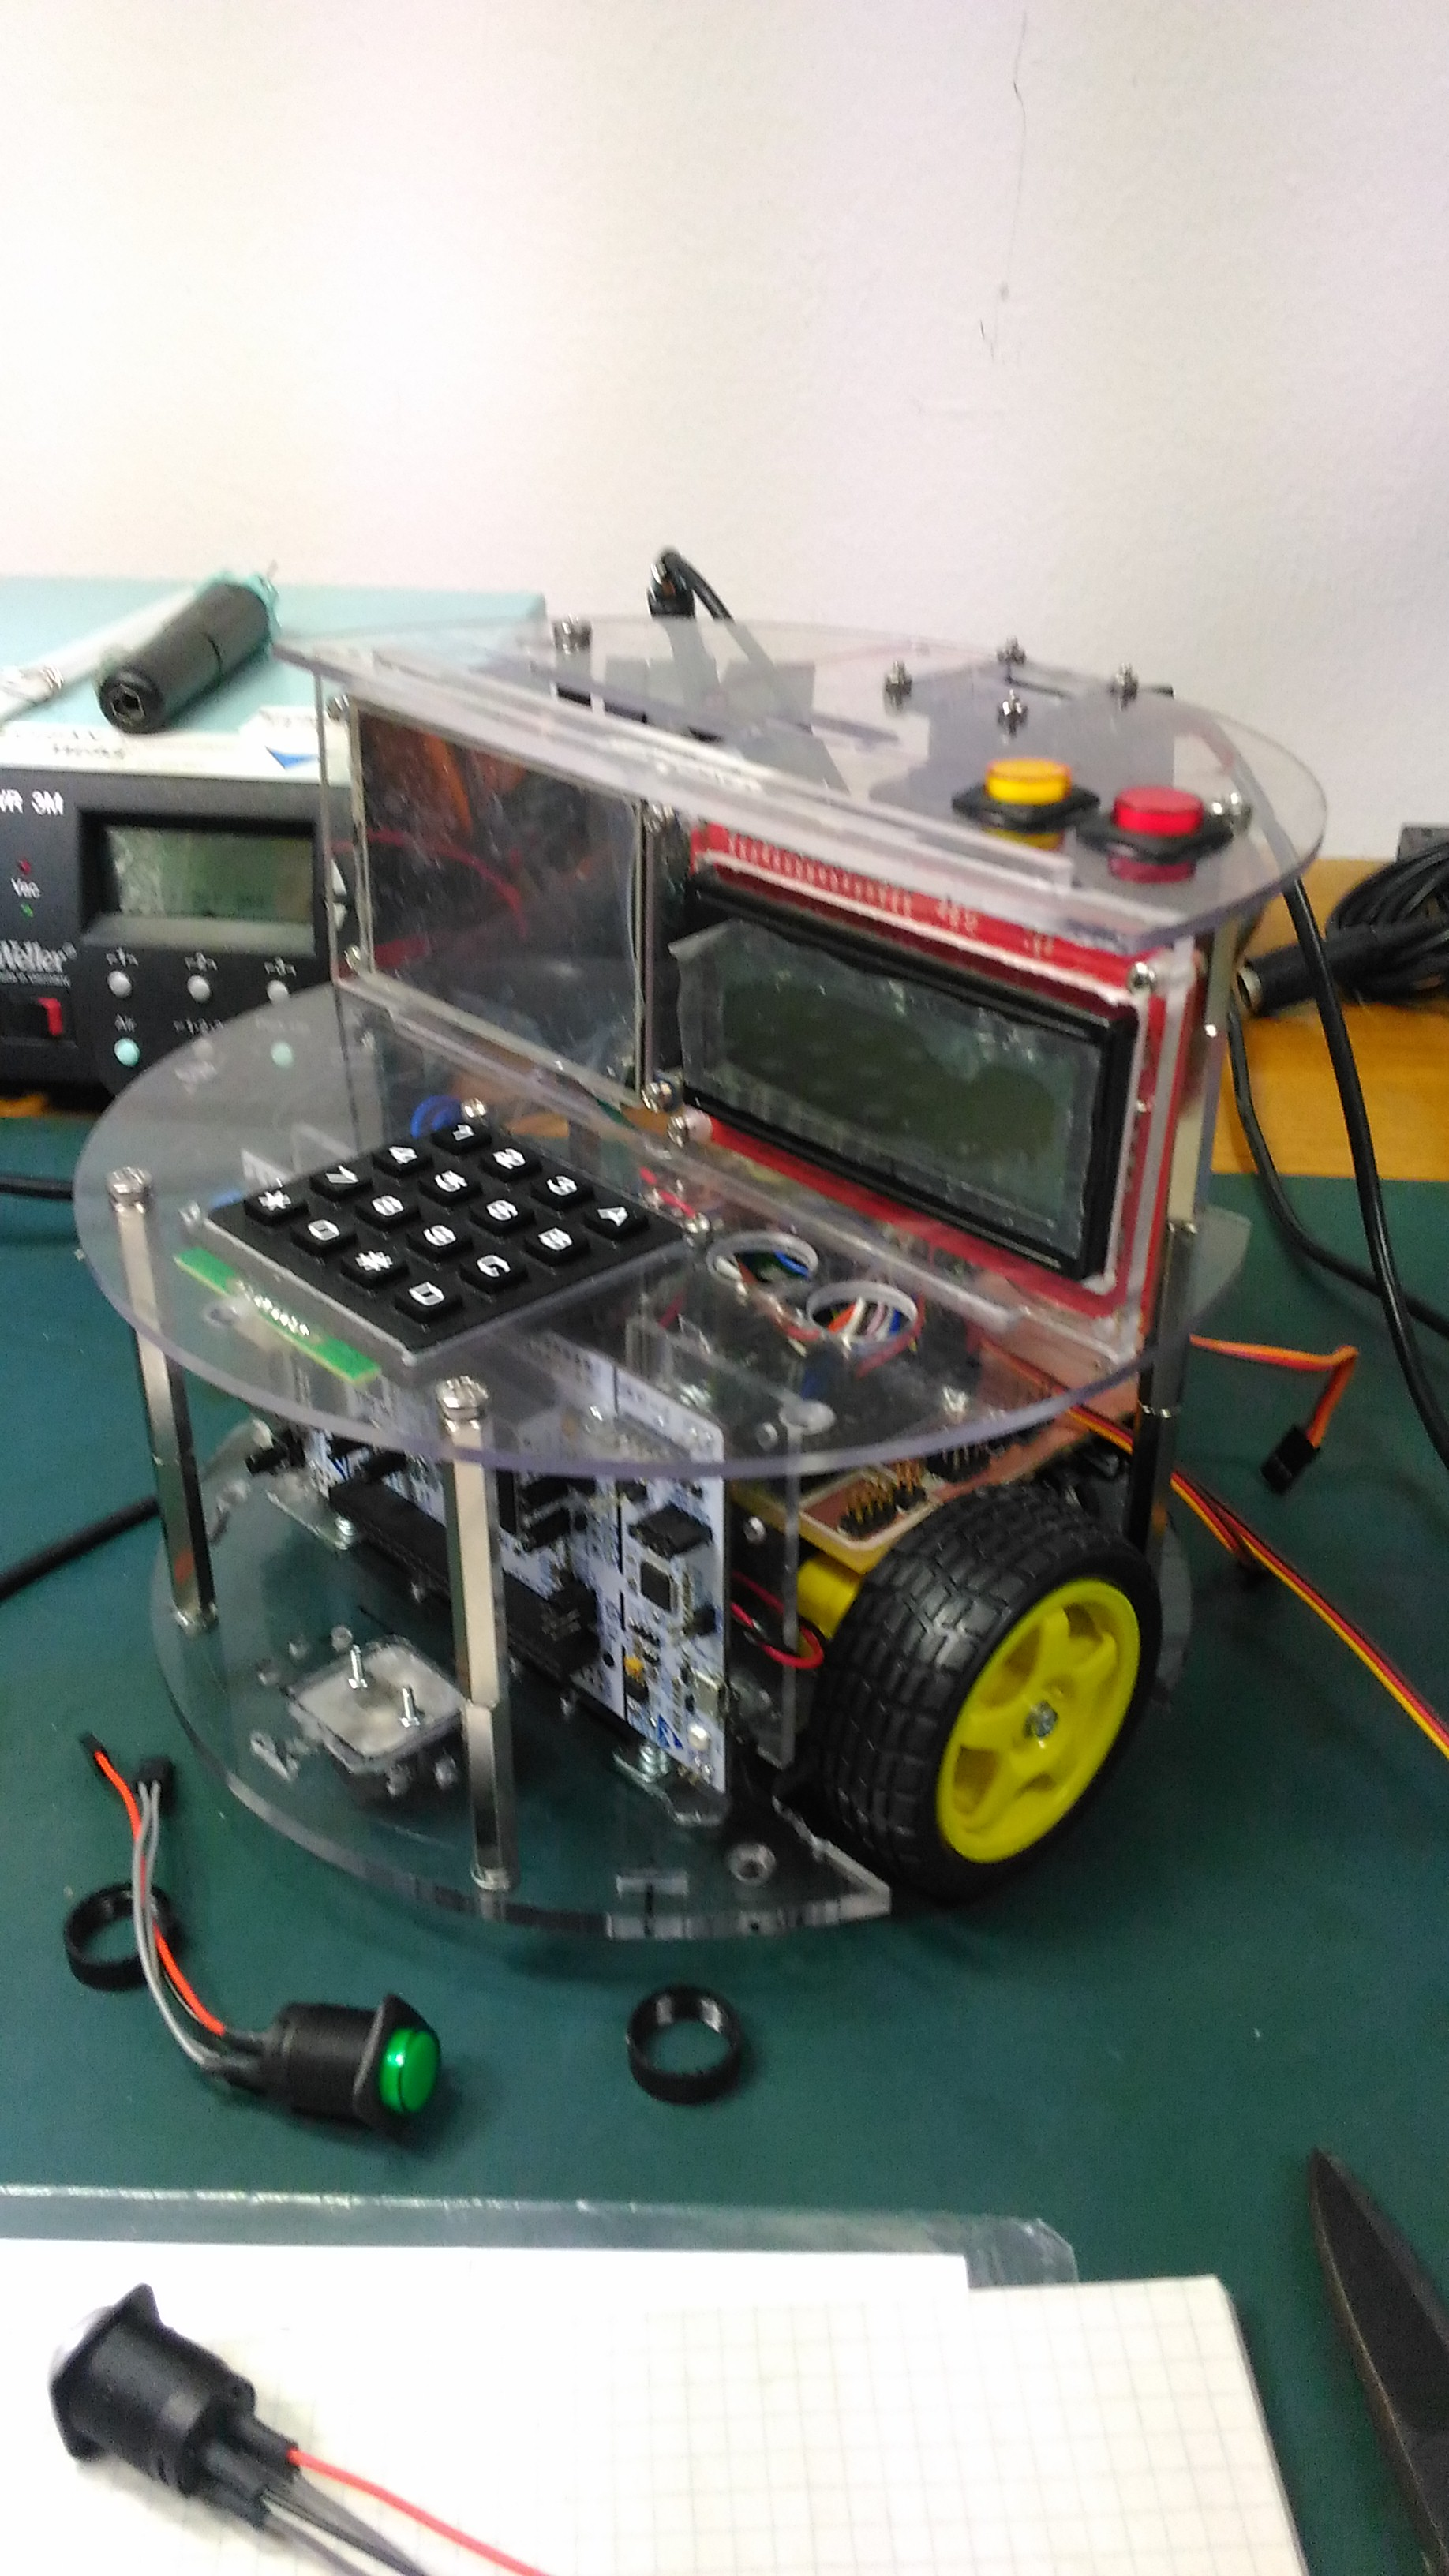
\includegraphics[width=0.4\textwidth]{figures/turtlebot_1.jpg}
	\caption{The TurtleBot}
	\label{fig:turtlebot}
\end{figure}

In Figure~\ref{fig:turtlebot} ...

\begin{figure}[!ht]
	\centering
	\subfloat[The TurtleBot 1 ]
	{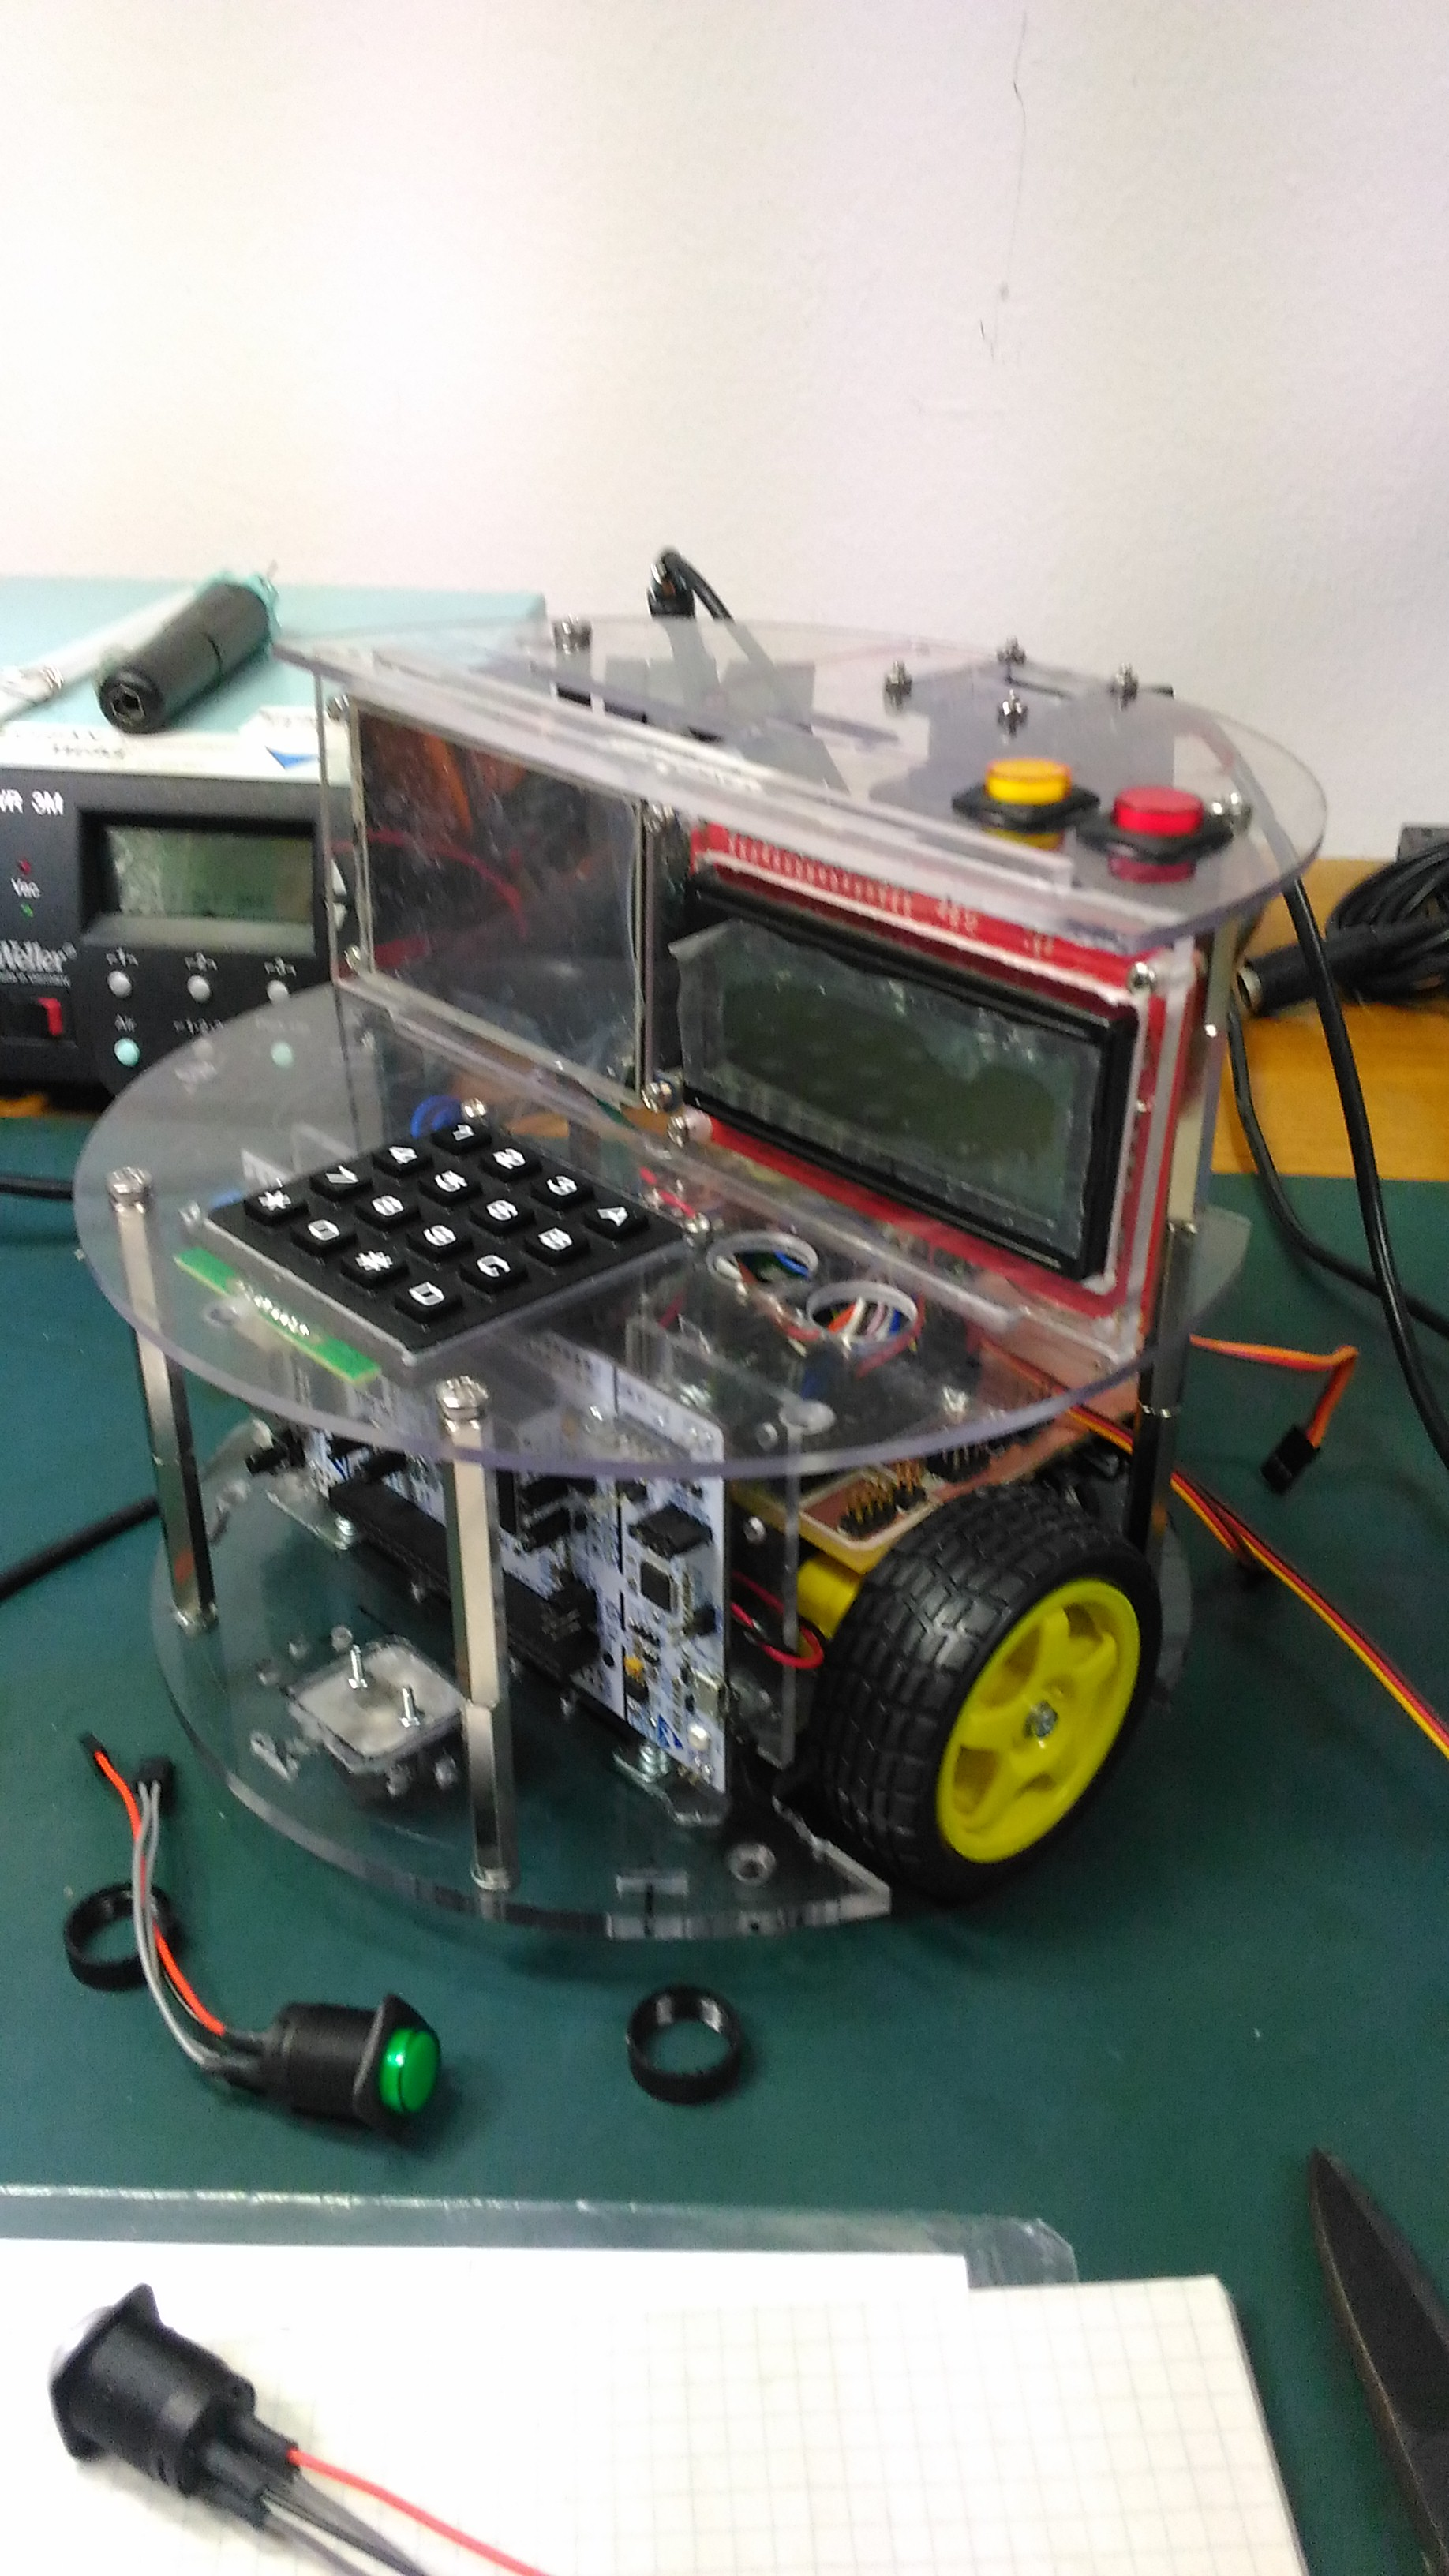
\includegraphics[width=0.3\textwidth,height=0.45\textwidth]{figures/turtlebot_1.jpg}
		\label{fig:tbot1}}
	\subfloat[The TurtleBot 2]
	{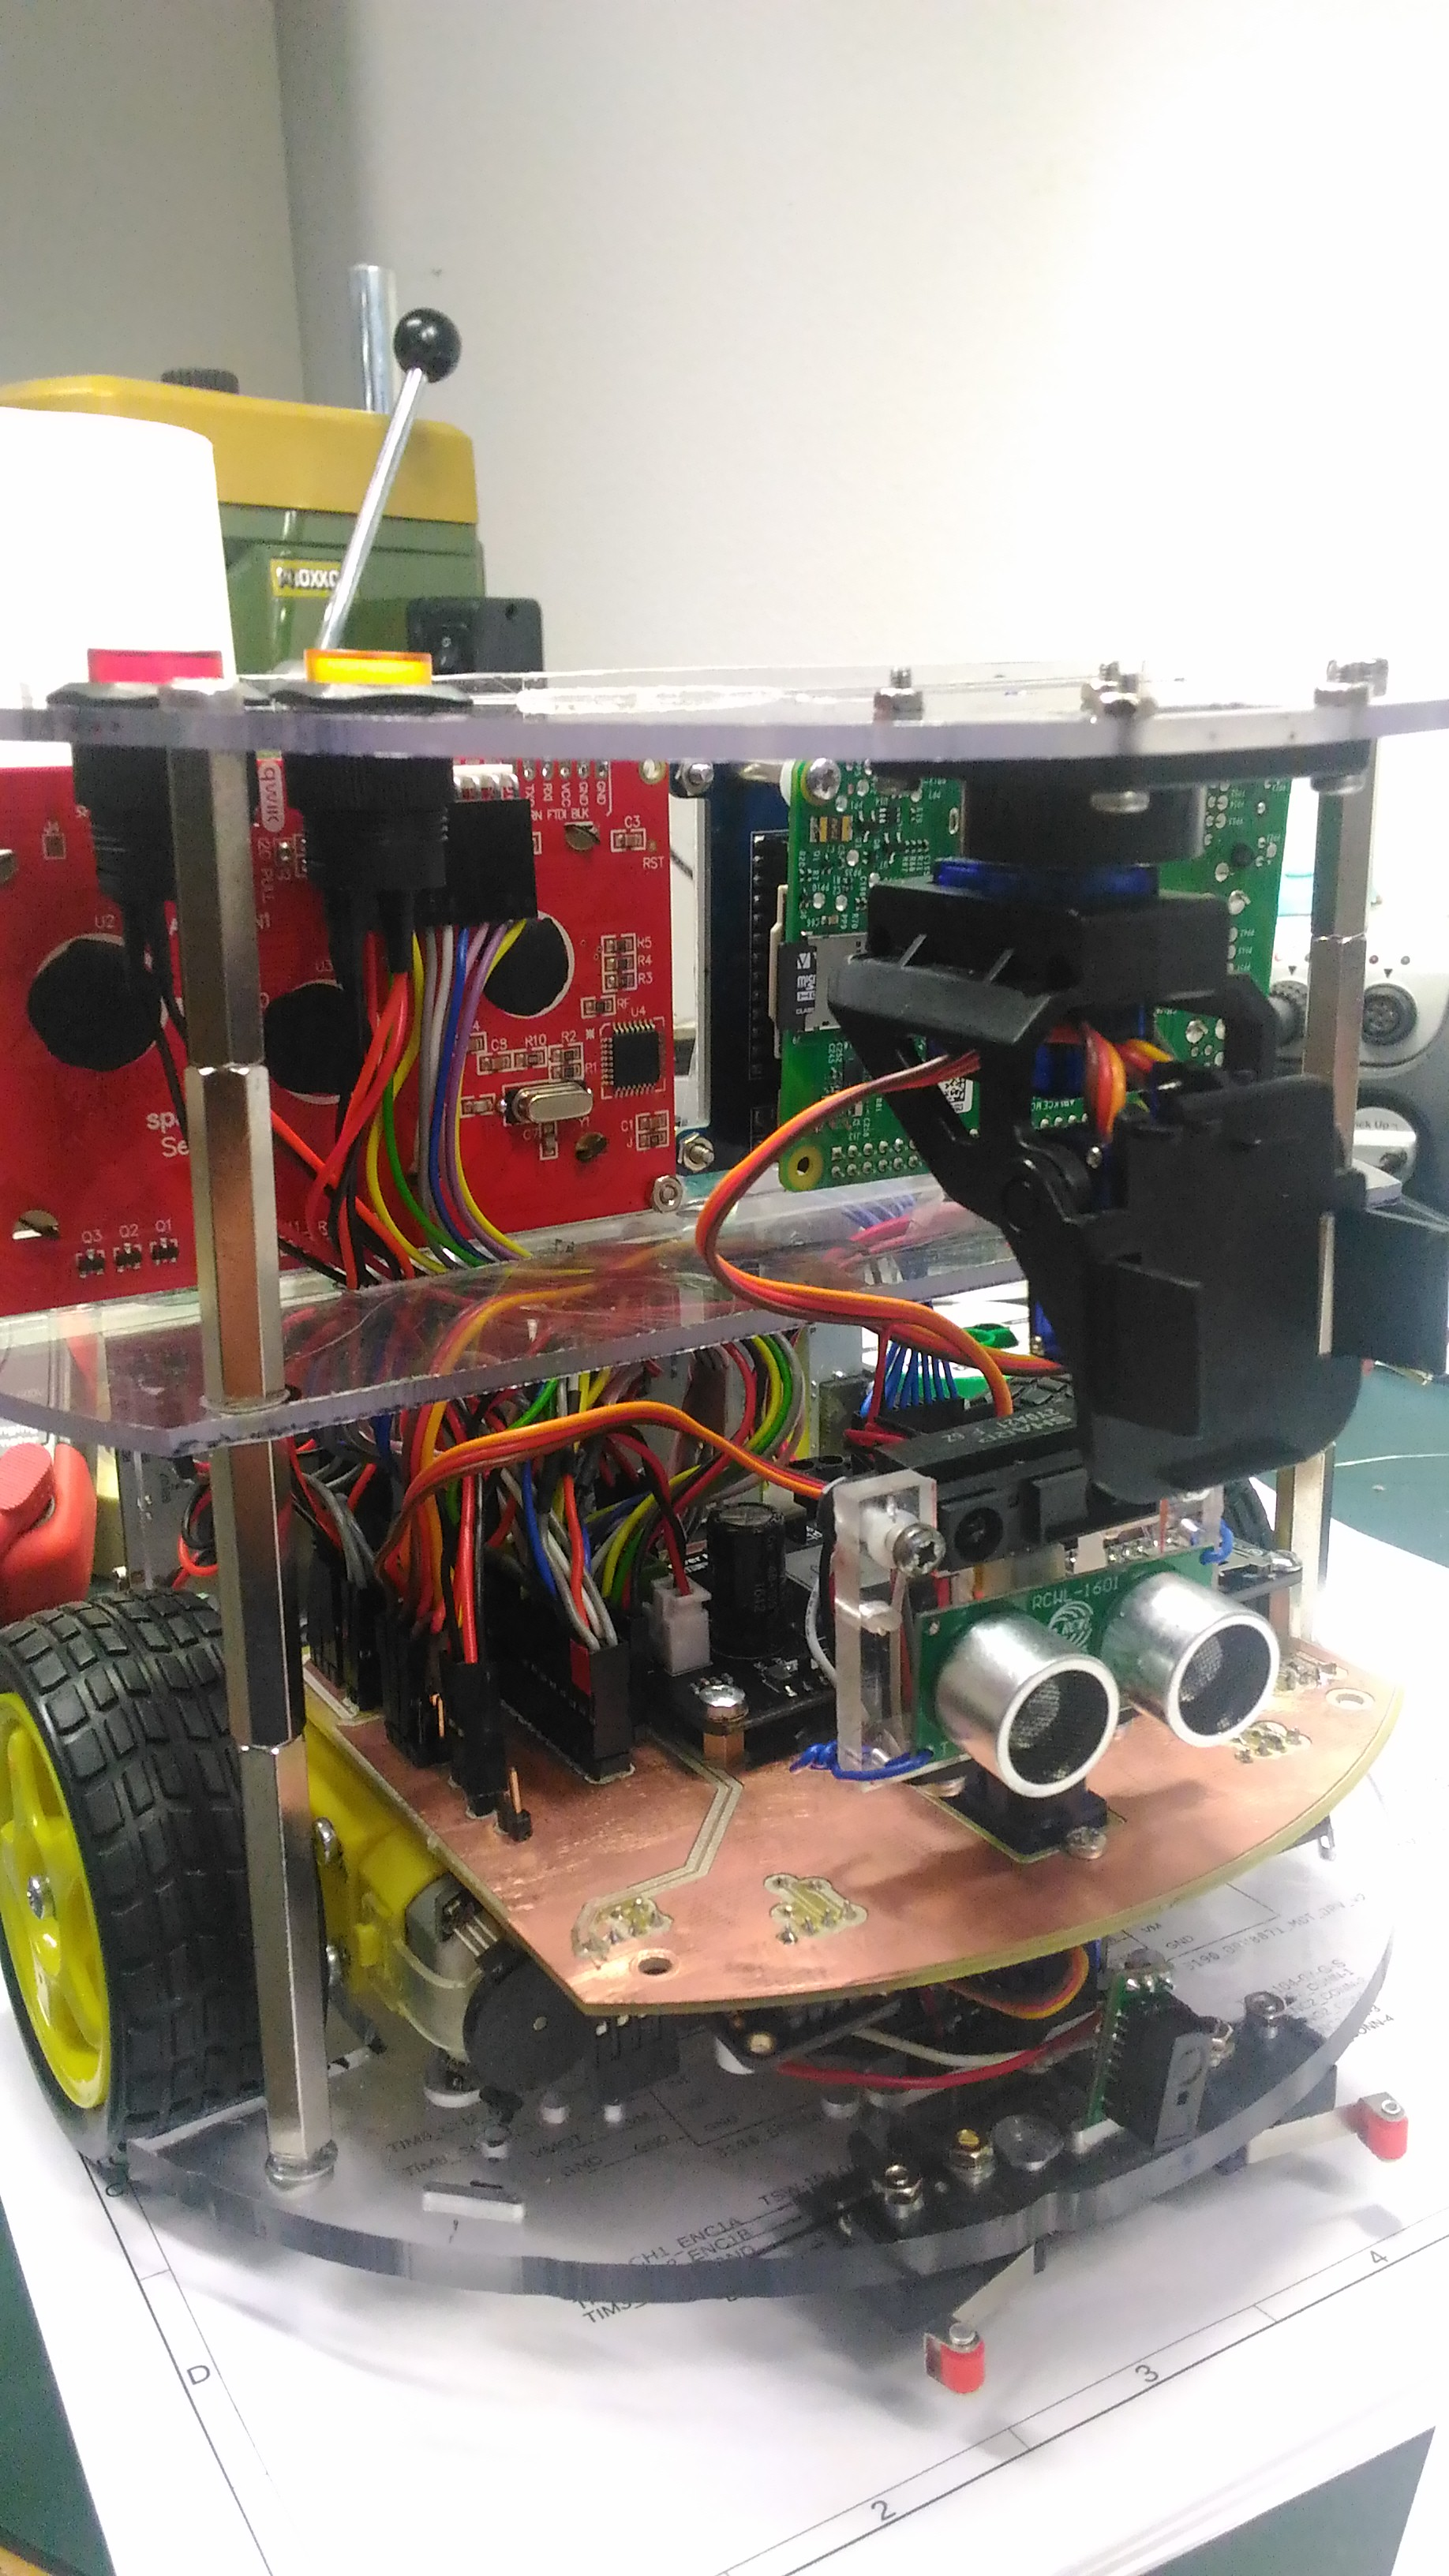
\includegraphics[width=0.3\textwidth,height=0.5\textwidth]{figures/turtlebot_2.jpg}
		\label{fig:tbot2}}
	\caption{The TurtleBot}
\end{figure}

\subsection{Another subsection}

Lorem ipsum dolor sit amet, consectetur adipisci elit, sed eiusmod tempor incidunt ut labore et dolore magna aliqua. Ut enim ad minim veniam, quis nostrum exercitationem ullam corporis suscipit laboriosam, nisi ut aliquid ex ea commodi consequatur.

\subsection{Another subsection}

\begin{lstlisting}[language=C, caption={C code using listings}, label={lst:label} ]
#include <stdio.h>
int main()
{
	// print hello to the console
	printf("Hello, world!");
	return 0;
}
\end{lstlisting}

See code~\ref{lst:label}.




\clearpage
\appendix

\section{Section in the Appendix}
\label{sec:app1}

\subsection{Subsection in the Appendix}
\label{subsec:app2}

Additional relevant information...

\end{document}